\section{Alternate Objective for Tractability}


\subsection{Motivation}

The original problem formulation we mentioned above encapsulates all
the semantic properties that we would like the obtained solution to
have (flow similarity, labelling coherence etc.). However, when we
consider the problem of finding $\underset{W}{argmin}f_{I}(X,W)$
where $f_{I}(X,W)=\lambda_{1}A(X,I)+\lambda_{2}S(X)+\lambda_{3}T(X,W)+\lambda_{4}F(W,I)+\lambda_{5}C(W)+\lambda_{6}M(W)$,
we encounter the following difficulties -


\subsubsection*{Non-Convexity}

The momentum continuity penalty as defined above i.e. $M(W)=\underset{i,j,t}{\sum}\quad\underset{a,b\in\{-h,..,h\}}{\sum}W_{ijt}^{ab}(|a-\overline{U}_{i+a,j+b,t+1}|+|b-\overline{V}_{i+a,j+b,t+1}|)$
is non-convex w.r.t $W$ (beacause $U$ is linear w.r.t $W$ so $M(W)$
has a product of variables of $W_{t},W_{t+1}$).


\subsubsection*{Large Number of Variables}

The size of the variable $W$ is $(2h+1)^{2}*|I|$. For a reasonable
sized video segment, this value becomes more than $10^{7}$ even if
we downsample the video. This makes it very difficult to solve the
minimization problem of this order with limited computational resources
in a reasonable time.

\medskip{}


We had earlier observed that the variables $W$ and $(U,V)$ can be
approximated from each other. Since the size of $(U,V)$ is only $|I|$,
we can define penalty functions equivalent/similar to the above in
terms of $U,V$ instead of $W$.


\subsection{Brightness constancy assumption and Horn-Schunk algorithm}

Before we describe the reformulation of the original objective function,
we briefly describe a well established computer vision algorithm that
motivates and justifies the relaxations used by us. The Horn-Schunk
algorithm \cite{HornSchunk} addresses the problem of finding optical
flows i.e. given an image pair $(I_{1},I_{2}$), we want to find the
optical flow field ($U_{1},V_{1})$ for each pixel in $I_{1}$. They
use a first order approximation over image intensity values and therefore
use $(\frac{\partial I}{\partial x}u+\frac{\partial I}{\partial x}v+\frac{\partial I}{\partial t})$
as a proxy for the image intensity difference of a pixel in $I_{2}$
at the location $(u,v)$ away from the current pixel. Formally, the
Horn-Schunk algorithm minimizes the following objective -

\begin{equation}
E(U,V)=\underset{i,j}{\sum}[(\frac{\partial I}{\partial x}u+\frac{\partial I}{\partial y}v+\frac{\partial I}{\partial t})^{2}+\alpha^{2}(\|\Delta u\|^{2}+\|\Delta v\|^{2})]
\end{equation}


Here, $(\Delta u,\Delta v)$ are the spatial derivatives of the flow
field. Drawing the analogies between our original objective and the
objective in Horn-Schunk algorithm, we observe that the first term
$\underset{i,j}{\sum}[(\frac{\partial I}{\partial x}u+\frac{\partial I}{\partial x}v+\frac{\partial I}{\partial t})^{2}$
captures the Flow Similarity penalty (that the corresponding pixel
in the next frame should be similar). The terms $ $$(\|\Delta u\|^{2}+\|\Delta v\|^{2})$
represent the flow continuity (that neighboring pixels have similar
flow). For our problem, if we assume that $(\Delta u,\Delta v)$ the
spatial as well as the temporal derivatives of the flow field, we
can also capture the Momentum Continuity penalty. Note that using
penalties and first-order approximations similar to the Horn-Schunk
algorithm, we obtain a convex objective. also, we can formualte the
optimization problem in terms of the variables $U,V$ instead of $W$
and achieve a huge reduction in terms of the number of variables.
We also see that if we use the $L1$ norm penalty instead of the $L2$
norm, we can obtain an $LP$ using auxillary variables. These minor
modifications to the original objective fnuction help us retain the
original penalties while obtaining a formulation with a much lower
complexity than the original one.


\subsection{Reformulated problem}

We incoorporate the relaxations motivated by the Horn-Schunk algorithm
and modify penalties to make an $LP$ formulation feasible. The final
minimization problem that we obtain is as follows -


\subsubsection*{Objective}

\begin{equation}
\underset{X,W}{\min}\enskip\lambda_{1}A'(X,I)+\lambda_{2}S'(X)+\lambda_{3}T'(X,W)
\end{equation}
\[
+\lambda_{4}F'(W,I)+\lambda_{5}[C'(W)+M'(W)]
\]


\begin{center}
subject to $W\geq0,\forall(i,j,t)X_{ijt}\in\{0,1\},\underset{a,b}{\sum}W_{ijt}^{ab}=1$
and $\forall t\underset{i,j}{|\sum}X_{ijt}-\underset{i,j}{\sum}X_{ij(t+1)}|\leq\sigma\underset{i,j}{\sum}X_{ijt}$ 
\par\end{center}

\noindent The objective function comprises of various penatly terms
which are explained below. The last constraint specifies that the
number of foreground pixels in do not change rapidly between consecutive
frames.

\subsubsection*{Appearance Model $A'(X,I)$}

We compute an object model using the segmentation in the first frame.
Using this, we pre-compute a cost matrix MA which determines the cost
between $[0,1]$ of a pixel $(i,j,t)$ being a foreground pixel. Once
precomputed, this cost matrix $A$ is fixed for the subsequent stages
of the optimization. The appearance cost is then computed as follows
-

\begin{equation}
A'(X,I)=\underset{i,j,t}{\sum}A_{i,j,t}*X_{ijt}+(1-A_{i,j,t})*(1-X_{ijt})
\end{equation}



\subsubsection*{Spatial Labelling Coherence $S(X)$}

\begin{equation}
S'(X)=S(X)=\underset{i,j,t}{\sum}\quad\underset{Y\in N_{s}(i,j,t)}{\sum}|X_{ijt}-X_{Y}|
\end{equation}



\subsubsection*{Flow Similarity $F(W,I)$}

\begin{equation}
F'(W,I)=F(U,V,I)=\underset{i,j,t}{\sum}|\frac{\partial I}{\partial x}U_{i,j,t}+\frac{\partial I}{\partial y}V_{i,j,t}+\frac{\partial I}{\partial t}|
\end{equation}


\subsubsection*{Temporal Labelling Coherence $T(X,W)$}

Similar to the firsr order approximation to the intersity field $I$,
we can also make a first order approximation to the label value field
$X$. This gives us the following penalty -

\begin{equation}
T'(X,W)=T(X,U,V)=\underset{i,j,t}{\sum}|\frac{\partial X}{\partial x}U_{i,j,t}+\frac{\partial X}{\partial y}V_{i,j,t}+\frac{\partial X}{\partial t}|
\end{equation}



\subsubsection*{Flow Continuity $C(W)$ + Momentum Continuity $M(W)$}

\begin{equation}
C'(W)+M'(W)=\underset{i,j,t}{\sum}\|\Delta u\|_{1}+\|\Delta v\|_{1}
\end{equation}

\begin{figure*}[t]
\begin{centering}
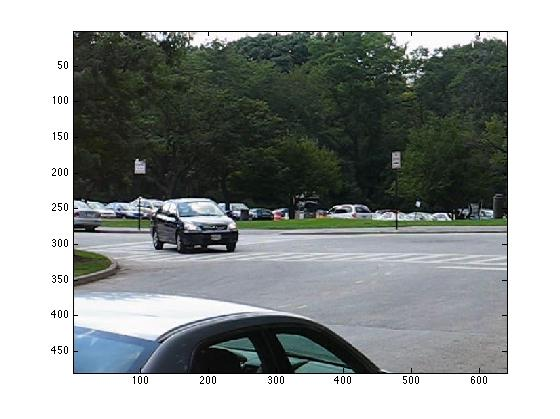
\includegraphics[scale=0.4]{figures/UnaryCostGT}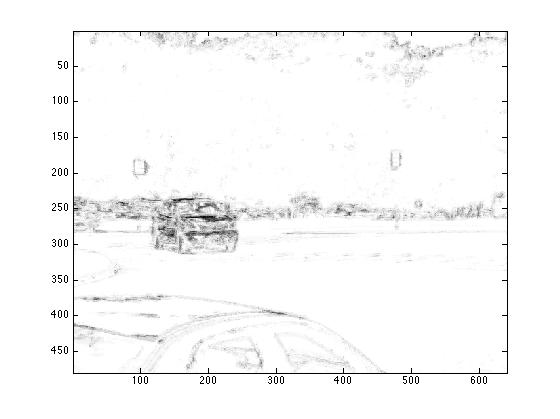
\includegraphics[scale=0.4]{figures/UnaryCost}\caption{Appearance Costs visualization : Low intensity represents low foreground cost
(object being tracked is upper car)}
\par\end{centering}
\end{figure*}

